\chapter{Phương pháp đề xuất}
\label{Chapter3}

% Trong chương này, khóa luận khảo sát hai và phân tích về ML và PL - hai hướng tiếp cận giúp cải thiện hiệu suất của hệ thống FL trên dữ liệu Non-IID. Từ đó đề xuất thuật toán \codeword{FedMeta-Per}, là sự kết hợp của hai kỹ thuật ML và PL vào hệ thống FL.

Trong chương này, khóa luận khảo sát bốn thuật toán chính bao gồm \codeword{FedMeta(MAML)}, \codeword{FedMeta(Meta-SGD)} trong nghiên cứu \cite{chen2018federated} (tích hợp phương pháp huấn luyện của các thuật toán ML vào hệ thống FL) và \codeword{FedPer}, \codeword{LG-FedAvg} trong các nghiên cứu \cite{arivazhagan2019federated}, \cite{liang2020think} (sử dụng kỹ thuật PL trong tối ưu độ chính xác và khả năng cá nhân hóa của hệ thống FL), giúp tạo hình thuật toán đề xuất \codeword{FedMeta-Per}. Từ đó, tiến đến phân tích sự kết hợp của bốn thuật toán này trong \codeword{FedMeta-Per}.

\section{Thuật toán $FedMeta(MAML)$ và $FedMeta(Meta-SGD)$}

\subsection{Thuật toán $FedMeta(MAML)$}

Nghiên cứu \cite{chen2018federated} đề xuất kết hợp \codeword{MAML} và \codeword{Meta-SGD} vào hệ thống FL của họ (thuật toán \ref{alg:fedmeta}). Tuy nhiên, tác giả sử dụng kỹ thuật cập nhật bằng cách lấy trung bình đạo hàm của hàm lỗi. Trước hết, máy khách sau khi nhận được trọng số toàn cục sẽ tiến hành fine-tune trọng số này trên tập dữ liệu support (phương trình \ref{eq:fine-tune_maml} và \ref{eq:fine-tune_metasgd}). Như vậy, mô hình sau khi fine-tune sẽ nắm bắt được các đặc trưng riêng của bộ dữ liệu. Từ đó thích ứng tốt với dữ liệu query.

\begin{dmath}
    \label{eq:fine-tune_maml}
    \text{MAML: } \hat{w}_i^{t+1} \gets w_G^t - \alpha\nabla_{w_G^t} f_{local}(w_G^t, \mathcal{D}_{train(i)}^{support})
\end{dmath}

\begin{dmath}
    \label{eq:fine-tune_metasgd}
    \text{Meta-SGD: } \hat{w}_i^{t+1} \gets w_G^t - \alpha^t \circ \nabla_{w_G^t} f_{local}(w_G^t, \mathcal{D}_{train(i)}^{support})
\end{dmath}

\begin{algorithm}[H]
    \caption{FedMeta(MAML) và FedMeta(Meta-SGD) \cite{chen2018federated}} \label{alg:fedmeta}
    \begin{algorithmic}[1]
        \State \textbf{Server:}
        \State Khởi tạo $w_G^0$ cho MAML hoặc ($w_G^0, \alpha^0$) cho Meta-SGD.
        \For{$t=0,1,2,...$}
            \State Chọn một tập $C_t$ gồm $m$ máy khách
            \For{$c_i \in C_t$}
                \State Tính toán $g_i^{t+1} \gets$ ModelTrainingMAML($c_i, w_G^t$) cho MAML
                \State Tính toán $g_i^{t+1} \gets$ ModelTrainingMetaSGD($c_i, w_G^t, \alpha^t$) cho Meta-SGD
            \EndFor

            \State

            \State Tính toán {$n_i = \left| \mathcal{D}_{train(i)}^{query} \right|, N_m = \sum_{i=0}^m n_i$}
            \State Cập nhật $w_G^{t+1} \gets w_G^t - \beta \sum_{i=0}^m \frac{n_i}{N_m} g_i^{t+1}$ cho MAML
            \State Cập nhật $(w_G^{t+1}, \alpha^{t+1}) \gets (w_G^t, \alpha^t) - \beta \sum_{i=0}^m \frac{n_i}{N_m} g_i^{t+1}$ cho Meta-SGD
        \EndFor

        \Statex

        \State\textbf{ModelTrainingMAML($c_i, w_G^t$):} \Comment{Tại máy khách $c_i$}
        \State Chọn tập support $\mathcal{D}_{train(i)}^{support}$ và tập query $\mathcal{D}_{train(i)}^{query}$
        \State $\hat{w}_i^{t+1} \gets w_G^t - \alpha\nabla_{w_G^t} f_{local}(w_G^t, \mathcal{D}_{train(i)}^{support})$
        \State $g_i^{t+1} \gets \nabla_{w_G^t} f_{local}(\hat{w}_i^{t+1}, \mathcal{D}_{train(i)}^{query})$
        \State Gửi $g_i^{t+1}$ về máy chủ

        \Statex

        \State\textbf{ModelTrainingMetaSGD($c_i, w_G^t, \alpha^t$):} \Comment{Tại máy khách $c_i$}
        \State Chọn tập support $\mathcal{D}_{train(i)}^{support}$ và tập query $\mathcal{D}_{train(i)}^{query}$
        \State $\hat{w}_i^{t+1} \gets w_G^t - \alpha^t \circ \nabla_{w_G^t} f_{local}(w_G^t, \mathcal{D}_{train(i)}^{support})$
        \State $g_i^{t+1} \gets \nabla_{(w_G^t,\alpha^t)} f_{local}(\hat{w}_i^{t+1}, \mathcal{D}_{train(i)}^{query})$
        \State Gửi $g_i^{t+1}$ về máy chủ
    \end{algorithmic}
\end{algorithm}

Trọng số sau khi fine-tune được dùng để dự đoán phân lớp trên tập dữ liệu query và tính toán hàm lỗi dựa trên kết quả dự đoán:

\begin{dmath}
    \label{eq:grad_maml}
    \text{MAML: } g_i^{t+1} \gets \nabla_{w_G^t} f_{local}(\hat{w}_i^{t+1}, \mathcal{D}_{train(i)}^{query})
\end{dmath}

\begin{dmath}
    \label{eq:grad_metasgd}
    \text{Meta-SGD: } g_i^{t+1} \gets \nabla_{(w_G^t,\alpha^t)} f_{local}(\hat{w}_i^{t+1}, \mathcal{D}_{train(i)}^{query})
\end{dmath}

Kết quả đạo hàm trên được gửi trực tiếp về máy chủ để tổng hợp bộ trọng số toàn cục mới:

\begin{dmath}
    \label{eq:agg_fedmetamaml}
    \text{MAML: } w_G^{t+1} \gets w_G^t - \beta \sum_{i=0}^m \frac{n_i}{N_m} g_i^{t+1}
\end{dmath}

\begin{dmath}
    \text{Meta-SGD: } (w_G^{t+1}, \alpha^{t+1}) \gets (w_G^t, \alpha^t) - \beta \sum_{i=0}^m \frac{n_i}{N_m} g_i^{t+1}
\end{dmath}

Khác với phương pháp tổng hợp nêu trên, khóa luận sử dụng kỹ thuật lấy trung bình trọng số trong việc tổng hợp trọng số toàn cục vì chi phí giao tiếp của việc truyền thông tin đạo hàm từ máy khách về máy chủ vượt quá giới hạn phần cứng được cung cấp. Đặt trong ngữ cảnh của ML, nếu bỏ qua việc mất gói tin trong quá trình giao tiếp giữa máy chủ và máy khách, việc sử dụng trọng số để truyền tin không ảnh hưởng đến kết quả của bài toán và được chứng minh đối với \codeword{MAML} như sau:

Tại bước huấn luyện toàn cục thứ $t$ với sự tham gia của $m$ máy khách, phương trình \ref{eq:agg_fedmeta} trở thành:

\begin{dmath}
    \label{eq:prof}
    w_G^{t+1} = \sum_{i=1}^m{\frac{n_i}{N_m}\left[ w_i^t - \beta \left( I - \alpha \nabla^2 f_{local}(w_i^t) \right) \times \nabla f_{local}\left( w_i^t - \alpha\nabla f_{local}(w_i^t)\right) \right]}
        = w_G^t - \beta \sum_{i=1}^m \frac{n_i}{N_m} \left( I - \alpha \nabla^2 f_{local}(w_i^t) \right) \times \nabla f_{local}\left( w_i^t - \alpha\nabla f_{local}(w_i^t)\right)
        = w_G^t - \beta \sum_{i=1}^m \frac{n_i}{N_m} g_c^{t+1}
\end{dmath}

Từ phương trình \ref{eq:prof} và \ref{eq:agg_fedmetamaml}, ta suy ra điều cần chứng minh. Đối với \codeword{Meta-SGD} và các bước thực hiện như trên, ta thu được kết quả chứng minh tương tự.

\subsection{Thuật toán $FedMeta(Meta-SGD)$}

Về phần thuật toán \codeword{Meta-SGD}, nghiên cứu \cite{li2017meta} chỉ ra rằng việc sử dụng một siêu tham số học cục bộ nhỏ, được cố định theo thời gian hoặc một một siêu tham số cục bộ giảm dần theo thời gian chỉ phù hợp cho ngữ cảnh huấn luyện một mô hình với bộ dữ liệu lớn trong thười gian dài. Trong ngữ cảnh dữ liệu gắn nhãn có ít nhưng mô hình cần phải thích ứng nhanh với tập dữ liệu mới, phương pháp chọn siêu tham số như vậy không còn phù hợp nữa.

Nghiên cứu cũng đề ra một hướng tiếp cận mới cho phép tự điều chỉnh và tối ưu siêu tham số cục bộ. Theo đó, ngoài việc tối ưu tri thức tiên nghiệm ($\omega$), thuật toán coi siêu tham số học tại cấp thấp $\alpha$ cũng là một tham số có thể tối ưu. Bằng việc khởi tạo $\alpha$ là một mảng siêu tham số có kích thước giống như $w$, thuật toán hướng tới việc cập nhật cả hướng đi lẫn bước học cho từng phần tử trọng số trong $w$ bằng cách điều chỉnh $\alpha$ tại bước tối ưu cấp cao. Máy khách sau đó sử dụng $\alpha$ bằng cách nhân vô hướng đại lượng này với đạo hàm hàm lỗi cục bộ. Xét trong quan hệ với hệ thống FL, \codeword{Meta-SGD} vừa khiến cho các mô hình học thích ứng nhanh trên các tập dữ liệu cục bộ, vừa đóng góp lớn vào việc cá nhân hóa mô hình học cho từng người dùng.

\section{Thuật toán $FedPer$ và $LG-FedAvg$}

% trình bày về FedPer
% trình bày về LG-FedAvg
% nhận xét về ưu nhược điểm của 2 thằng
% chỉ ra cách kết hợp của 2 thằng (lấy 2 cái ưu điểm: 1 thằng test được nhiều TH hơn, 1 thằng đạt độ chính xác cao hơn)

\subsection{Thuật toán $FedPer$}

Nghiên cứu \cite{arivazhagan2019federated} đề xuất kiến trúc hệ thống FL theo hướng PL bằng cách chia mạng học sâu ra làm hai phần. Phần chung được hợp tác huấn luyện bởi các máy khách trong hệ thống và được tổng hợp bởi máy chủ. Phần riêng được các máy khách độc lập huấn luyện trên dữ liệu của mình (Hình \ref{fig:fedper}).

\begin{figure}[H]
    \centering
    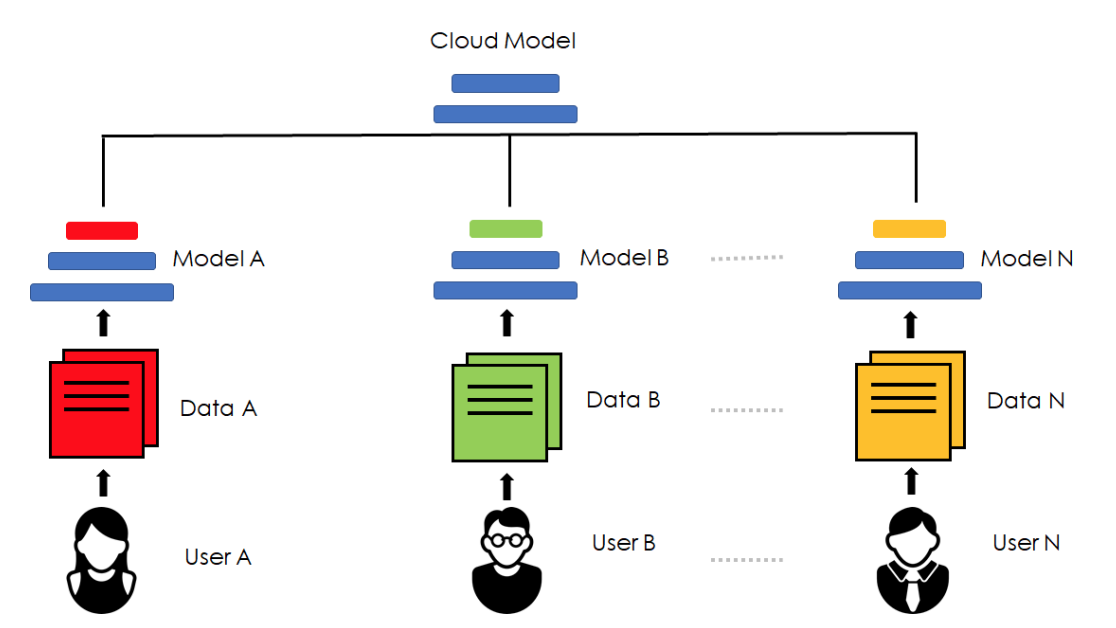
\includegraphics[scale=0.8]{../images/perlayer.png}
    \caption{Minh họa thuật toán FedPer \cite{arivazhagan2019federated}}
    \label{fig:fedper}
\end{figure}

Các lớp học sâu trong phần chung là các lớp rút trích đặc trưng của mạng. Vì được hợp tác huấn luyện, các lớp phần chung này được tiếp xúc với đầy đủ các phân lớp dữ liệu. Do đó, sẽ có được khả năng rút trích được đặc trưng dữ liệu của tất cả các nhãn dữ liệu trong hệ thống. Điều này là rất quan trọng và là điểm khác biệt chính khi so sánh giữa \codeword{FedPer} và \codeword{LG-FedAvg}.

Phần riêng của mạng bao gồm các lớp tuyến tính ở mức cao. Phần này sẽ sử dụng các đặc trưng dữ liệu được rút trích ở trên để tính toán và quyết định một mẫu dữ liệu đầu vào sẽ thuộc phân lớp nào. Vì được duy trì riêng tại mỗi máy khách, các lớp phần riêng này được tối ưu riêng cho dữ liệu trên máy khách đó. Đây chính là điểm đáng giá của thuật toán \codeword{FedPer} khi nó giúp nắm bắt điểm riêng biệt trong phân phối dữ liệu của từng máy khách mà thuật toán \codeword{FedAvg} không thể nào làm được.

Ký hiệu $w_{P(i)}, w_B$ lần lượt là trọng số của các lớp phần riêng của máy khách $c_i$ và phần chung của hệ thống. Hàm phân lớp cần huấn luyện tại máy khách $c_i$ là $\hat{y}_i = g(x, w_B, w_{P(i)})$. Trong đó, trọng số $w_B$ có nhiệm vụ rút trích các đặc trưng của dữ liệu đầu vào $x$ còn $w_{P(i)}$ chịu trách nhiệm phân lớp dữ liệu $x$ cũng như lưu trữ tính cá nhân hóa của máy khách $c_i$. Theo đó, hàm mục tiêu của hệ thống có thể được biểu diễn:

\begin{dmath}
    \min_{w_B, w_{P(1)},...,w_{P(n)}} f_{global}(w_B, w_{P(1)},...,w_{P(n)}) = \min_{w_B, w_{P(1)},...,w_{P(n)}} \frac{1}{n} \sum_{i=1}^n f_{local}(w_B, w_{P(i)})
\end{dmath}

Các hoạt động chính của máy chủ và máy khách trong hệ thống được trình bày trong thuật toán \ref{alg:fedper_server} và \ref{alg:fedper_client}. Đầu tiên, máy chủ khởi tạo trọng số phần chung $w_B^0$ và gửi trọng số này đến các máy khách trong một bước huấn luyện. Máy khách $c_i$ nhận $w_B^0$ từ máy chủ đồng thời khởi tạo trọng số phần riêng $w_{P(i)}^0$. Bộ trọng số $(w_B^0, w_{P(i)}^0)$ sau đó được máy khách $c_i$ sử dụng để dự đoán và huấn luyện cục bộ. Tại bước huấn luyện toàn cục thứ $t$, ta có:

\begin{equation}
    H = h(x, w_{B}^t)
\end{equation}
\begin{equation}
    \hat{y} = g(H, w_{P(i)}^t)
\end{equation}
\begin{equation}
    w_{B(i)}^{t+1} \leftarrow w_B^t - \alpha\nabla_{w_B^t} f_{local}(x, w_B^t, w_{P(i)}^t)
\end{equation}
\begin{equation}
    w_{P(n)}^{t+1} \leftarrow w_{P(n)}^t - \alpha\nabla_{w_{P(n)}^t} f_{local}(x, w_B^t, w_{P(n)}^t)
\end{equation}

Kết thúc quá trình huấn luyện cục bộ, $w_{P(n)}^{t+1}$ được lưu trữ lại còn $w_{B(i)}^{t+1}$ được gửi về máy chủ để tổng hợp $w_{B}^{t+1}$:

\begin{equation}
    w_B^{t+1} = \sum_{i=1}^n{\frac{n_i}{N}w_{B(i)}^{t+1}}
\end{equation}

\begin{algorithm}
    \caption{FEDPER-CLIENT($c_i, w_B^t$) \cite{arivazhagan2019federated}} \label{alg:fedper_client}
    \begin{algorithmic}[1]
        % \Require $f(.;.,.),e,b,\{(x_{j,i}, y_{j,i}) | i \in \{1,...n_j\}\}$
        \Require Siêu tham số học $\alpha$, trọng số $w_B^t$ từ máy chủ
        \If {$t=0$}
            \State Khởi tạo $w_{P(i)}^t$
        \Else
            \State Tải lại $w_{P(i)}^t$ đã được lưu trữ trước đó
        \EndIf
        \State Dự đoán: $H = h(x, w_{B}^t)$; $\hat{y} = g(H, w_{P(i)}^t)$
        \State Tính toán $(w_{B(i)}^{t+1}, w_{P(i)}^{t+1}) \gets (w_{B}^t, w_{P(i)}^t) - \alpha\nabla_{(w_{B}^t, w_{P(i)}^t)} f_{local}(w_{B}^t, w_{P(i)}^t, \mathcal{D}_i)$
        \State Gửi $w_{B(i)}^{t+1}$ về máy chủ và lưu trữ $w_{P(i)}^{t+1}$
    \end{algorithmic}
\end{algorithm}

\begin{algorithm}
    \caption{FEDPER-SERVER \cite{arivazhagan2019federated}} \label{alg:fedper_server}
    \begin{algorithmic}[1]
        \State Khởi tạo $w_{B}^{0}$
        \For {$t=0,1,2,...$}
            \State Chọn một tập $C_t$ gồm $m$ máy khách
            \For{ $c_i\in C_t$}
                \State Tính toán $(w_{B(i)}^{t+1}, n_i) \gets \text{FEDPER-CLIENT}(c_i, w_B^t)$
            \EndFor
            \State Tính toán $n_i = \left| \mathcal{D}_i \right|, N_m = \sum_{i=1}^m n_i$
            \State Cập nhật $w_B^{t+1} \gets \sum_{i=1}^m \frac{n_i}{N_m} w_{B(i)}^{t+1}$
        \EndFor
    \end{algorithmic}
\end{algorithm}

Sau khi hoàn thành giai đoạn huấn luyện toàn cục, hệ thống thu được một trọng số phần chung và $n$ trọng số phần riêng. Quá trình kiểm thử trên tập dữ liệu của máy khách mới được tiến hành bằng thông qua bộ tham số $(w_B, w_P)$. Trong đó, $w_P$ là trung bình cộng của các trọng số $(w_{P(1)},...,w_{P(n)})$, được tính bằng phương trình \ref{eq:w_P}.

\begin{dmath}
    \label{eq:w_P}
    w_P = \sum_{i=1}^n \frac{n_i}{N}w_{P(i)}
\end{dmath}

% Một lần nữa, dựa trên quán trình lấy trung bình cộng, trọng số của hệ thống lại gặp phải vấn đề tương tự như \codeword{FedAvg}. Bộ trọng số $(w_{P(1)},...,w_{P(n)})$ có thể mang đến sự cá nhân hóa rất tốt trên các máy khách đã tồn tại từ lâu trong hệ thống; trọng số $w_B$ được hợp tác huấn luyện nên có thể đã "quen thuộc" hơn đối với dữ liệu thuộc các nhãn khác nhau nhưng vẫn khó tránh khỏi việc giảm hiệu suất trên dữ liệu Non-IID. Trên các máy khách vừa tham gia hệ thống, hai trọng số này sẽ gặp tình trạng tương tự như thuật toán \codeword{FedAvg}: Bị giảm hiệu suất nghiêm trọng trên dữ liệu Non-IID.

Một lần nữa, bộ trọng số $(w_{P(1)},...,w_{P(n)})$ vốn có tính cá nhân hóa rất cao cho từng người dùng, giờ đây được tính trung bình và đem kiểm thử trên tập dữ liệu mới. Đối với việc dữ liệu bị Non-IID mạnh, việc lấy trung bình này sẽ gặp tình trạng giống như thuật toán \codeword{FedAvg}: Bị giảm hiệu suất nghiêm trọng trên dữ liệu Non-IID. Hiện tượng tương tự cũng xảy ra với trọng số phần chung $w_B$ do trọng số này được huấn luyện theo phương pháp truyền thống và được tổng hợp bằng cách lấy trung bình cộng. Do đó, không có gì đảm bảo rằng nó sẽ hoạt động tốt trên dữ liệu Non-IID.

\subsection{Thuật toán $LG-FedAvg$}

Ngoại trừ việc phần chung của mạng học sâu là các lớp tuyến tính còn phần riêng của mạng là các lớp rút trích đặc trưng, ý tưởng huấn luyện của thuật toán \codeword{LG-FedAvg} (thuật toán \ref{alg:lg_fedavg}) gần như giống hoàn toàn với thuật toán \codeword{FedPer}. Các lớp phần riêng của thuật toán này được kỳ vọng sẽ học những đặc trưng dữ liệu của từng máy khách một cách riêng biệt. Tuy nhiên, khi đối mặt với các phân phối dữ liệu lạ trên các máy khách vừa tham gia vào hệ thống, các lớp phần riêng tỏ ra khó khăn trong việc nắm bắt các đặc trưng mới vì chúng đã được cá nhân hóa rất cao cho các đặc trưng cục bộ trước đó. Dẫn đến việc độ chính xác của hệ thống giảm từ 31\% đến 34\% khi hoạt động trên các máy khách mới khi so sánh với độ chính xác trên các máy khách cũ \cite{liang2020think}.

Điểm nổi bật được chú ý đến trong nghiên cứu này chính là kịch bản mà nó xây dựng trong quá trình kiểm thử rất phù hợp với các tình huống thực tế của một hệ thống client-server. Kịch bản kiểm thử của nghiên cứu \cite{liang2020think} chia người dùng ra làm hai loại: (1) - Người dùng cục bộ, (2) - Người dùng mới.

Đối với người dùng cục bộ, nghiên cứu cho rằng loại người dùng này đã tồn tại đủ lâu trong hệ thống để có thể xây dựng được một lớp cá nhân hóa cho chính nó. Khi làm việc với loại dữ liệu trên máy khách của họ, hệ thống biết chính xác nên sử dụng bộ trọng số nào là phù hợp nhất.

\label{ensemble_test}
Đối với người dùng mới, nghiên cứu giả định họ là những người vừa tham gia vào hệ thống. Do đó, hệ thống không thể biết được nên sử dụng trọng số nào để làm việc với phân phối dữ liệu của họ. Chính vì vậy, nghiên cứu đề xuất thực hiện ensemble test\footnote{Lớp phần chung được ghép với từng lớp phần riêng để tạo thành các mạng neuron riêng biệt. Các mạng này được dùng để kiểm thử trên dữ liệu. Kết quả cuối được đưa ra bằng hình thức bỏ phiếu.} trên loại người dùng này.

\begin{algorithm}[H]
    \caption{LG-FEDAVG \cite{liang2020think}}\label{alg:lg_fedavg}
    \begin{algorithmic}[1]
        \State \textbf{Server:}
        \State Khởi tạo $w_B^0$
        \For{$t=1,2,...$}
            \State Chọn một tập $C_t$ gồm $m$ máy khách
            \For{$c_i \in C_t$}
                \State Tính toán $w_{B(i)}^{t+1} \gets ClientUpdate(c_i,w_B^t)$
            \EndFor

            \State Tính toán $n_i = \left| \mathcal{D}_i \right|, N_m = \sum_{i=1}^m n_i$
            \State Cập nhật $w_B^{t+1} \gets \sum_{i=1}^m\frac{n_i}{N_m} w_{B(i)}^{t+1}$ %\COMMENT{// aggregate updates}
        \EndFor

        \Statex

        \State \textbf{ClientUpdate} $(c_i, w_B^t)$: %\COMMENT{// run on client $m$}
        \If {$t=0$}
            \State Khởi tạo $w_{P(i)}^t$
        \Else
            \State Tải lại $w_{P(i)}^t$ đã được lưu trữ trước đó
        \EndIf
        \State Dự đoán: $H = h(x, w_{P(i)}^t); \hat{y} = g(H, w_B^t)$
        \State Tính toán $(w_{B(i)}^{t+1}, w_{P(i)}^{t+1}) \gets (w_{B}^t, w_{P(i)}^t) - \alpha\nabla_{(w_{B}^t, w_{P(i)}^t)} f_{local}(w_{B}^t, w_{P(i)}^t, \mathcal{D}_i)$
        \State Gửi $w_{B(i)}^{t+1}$ về máy chủ và lưu trữ $w_{P(i)}^{t+1}$
    \end{algorithmic}
\end{algorithm}

Dựa trên việc phân chia dữ liệu theo hướng ML, khóa luận không đồng ý với cách tiếp cận ensemble test trên người dùng mới vì hai lý do. Thứ nhất, khả năng thích ứng trên tập dữ liệu mới của các lớp phần riêng của hệ thống bị triệt tiêu, thay vào đó là tính cá nhân hóa cho từng tập dữ liệu cục bộ mà hệ thống đã làm việc trước đó. Đứng trước một tập dữ liệu mới, các lớp phần riêng này hầu như không đạt được hiệu suất cao, dẫn đến kết quả của ensemble test không được như kỳ vọng. Thứ hai, cách tổ chức dữ liệu của hệ thống FL theo hướng ML yêu cầu chia tập dữ liệu cục bộ ra thành hai tập con (tập support và query). Mô hình học sẽ được thích ứng với dữ liệu kiểm tra thông qua một vài bước fine-tune trên tập support. Vì vậy, có thể chọn ra lớp phần riêng phù hợp nhất trong quá trình fine-tune. Do đó, dù hoạt động đơn lẻ hơn so với ensemble test, phương pháp này vẫn có khả năng đạt được độ chính xác thậm chí cao hơn phương pháp của nghiên cứu \cite{liang2020think} đề xuất.

% lý do 1: hệ thống tệ vcl r, ensemble thì cx là 1 đám ăn hại nc với nhau
% lý do 2: bên ML chia data theo kiểu có support và query trên tập test nên có thể mò ra thằng weight tốt nhất cho hệ thống dựa vào tập support này.
% việc duy trì 1 thằng per layer (do ML huấn luyện) nên được xem xét và thử nghiệm, do trên các weight hiện tại, khả năng gen trên tập data mới đang bị hạn chế (vì dù train theo ML nhưng lại k có tổng hợp)

\section{Thuật toán đề xuất: $FedMeta-Per$}

\subsection{Cấu trúc hệ thống}

Theo hướng tiếp cận PL, phương pháp đề xuất chia mạng học sâu ra thành hai phần. Phần chung bao gồm các lớp rút trích đặc trưng của mạng, được hợp tác huấn luyện bởi các máy khách và tổng hợp bởi máy chủ hệ thống. Phần riêng bao gồm các lớp tuyến tính còn lại, được duy trì tại mỗi máy khách, giúp tăng tính cá nhân hóa mô hình cho tập dữ liệu biên.

Điểm khác biệt giữa phương pháp này và thuật toán \codeword{FedPer} nằm ở chỗ các lớp của mạng học sâu thuộc phần chung được huấn luyện theo hướng ML. Do đó, thuật toán đề xuất được đặt tên là \codeword{FedMeta-Per} - sự kết hợp giữa các thuật toán \codeword{FedMeta} và thuật toán \codeword{FedPer}.

Trong ba phần dưới đây, khóa luận mô tả về cách thức mà hệ thống hoạt động trong quá trình huấn luyện (bao gồm huấn luyện cục bộ và tổng hợp toàn cục) và các kịch bản kiểm thử thuật toán.

\subsection{Huấn luyện cục bộ}

Giai đoạn huấn luyện cục bộ bằng cách sử dụng thuật toán \codeword{MAML} và \codeword{Meta-SGD} được trình bày trong thuật toán \ref{alg:fedmaml_per_client} và \ref{alg:fedsgd_per_client}. 

Đối với các máy khách huấn luyện theo thuật toán \codeword{MAML}, tại bước huấn luyện toàn cục thứ $t$, một máy khách $c_i$ ban đầu sẽ nhận được trọng số khởi tạo $w_B^t$ của phần chung do máy chủ gửi đến. Dưới hình thức huấn luyện của ML, $c_i$ cần phải chuẩn bị hai tập dữ liệu $\mathcal{D}_{train(i)}^{support}$ và $\mathcal{D}_{train(i)}^{query}$. Tiếp đến, $c_i$ tiến hành hợp nhất trọng số phần chung $w_B^t$ với trọng số phần riêng $w_{P(i)}^t$ (được khởi tạo ngẫu nhiên trong bước huấn luyện toàn cục đầu tiên và được tải lại trong các bước huấn luyện sau) để thu được trọng số của mô hình hoàn chỉnh $w_i^t$. $w_i^t$ sau đó được huấn luyện như sau:

\begin{dmath}
    \text{Train: } \hat{w}_{i}^{t+1} \gets w_{i}^t - \alpha\nabla_{w_i^t} f_{local}\left(w_{i}^t, \mathcal{D}_{train(i)}^{support}\right)
\end{dmath}

\begin{dmath}
    \text{Meta-train: } w_{i}^{t+1} \gets w_{i}^t - \beta\nabla_{w_i^t} f_{local}\left(\hat{w}_{i}^{t+1}, \mathcal{D}_{train(i)}^{query}\right)
\end{dmath}

Đối với các máy khách sử dụng thuật toán \codeword{Meta-SGD} trong huấn luyện, phần chung của mạng học sâu bao gồm hai tham số: trọng số huấn luyện chung $w_B^{t}$ và siêu tham số huấn luyện chung $\alpha_B^{t}$; phần riêng của mạng bao gồm hai tham số $w_{P(i)}^{t}$ và $\alpha_{P(i)}^{t}$. Quá trình hợp nhất tham số cũng được diễn ra giữa các tham số phần chung và phần riêng để tạo thành bộ tham số hoàn chỉnh $w_i^t$ và $\alpha_i^t$. Hai tham số này sau đó cũng tham gia vào quá trình huấn luyện giống như \codeword{MAML}:

\begin{dmath}
    \text{Train: } \hat{w}_{i}^{t+1} \gets w_{i}^t - \alpha_i^t\circ\nabla_{w_i^t} f_{local}\left(w_{i}^t, \mathcal{D}_{train(i)}^{support}\right)
\end{dmath}

\begin{dmath}
    \text{Meta-train: } (w_{i}^{t+1}, \alpha_i^{t+1}) \gets (w_{i}^t, \alpha_{i}^{t}) - \beta\nabla_{(w_i^t, \alpha_i^t)} f_{local}\left(\hat{w}_{i}^{t+1}, \mathcal{D}_{train(i)}^{query}\right)
\end{dmath}

Kết thúc quá trình huấn luyện cục bộ, trọng số mô hình mới $w_i^{t+1}$ được phân giải thành trọng số phần chung mới $w_{B(i)}^{t+1}$ và trọng số phần riêng mới $w_{P(i)}^{t+1}$. $w_{B(i)}^{t+1}$ được gửi về máy chủ để tổng hợp $w_B^{t+1}$ còn $w_{P(i)}^{t+1}$ được lưu lại tại bộ nhớ của máy khách. Việc phân giải, gửi về máy chủ và lưu trữ tham số tại máy khách cũng diễn ra tương tự với siêu tham số $\alpha_i^t$.

\textbf{Với việc sử dụng ML trong huấn luyện mạng học sâu cục bộ, trọng số phần chung toàn cục sẽ có được khả năng thích ứng nhanh trên tập dữ liệu mới của kỹ thuật ML. Từ đó, mạng học sâu của thuật toán đề xuất có thể dễ dàng nắm bắt các đặc trưng của người dùng mới trong hệ thống}. Đây chính là giải pháp cho câu hỏi về cách cải thiện các lớp phần chung của các thuật toán theo hướng PL được nên trong phần \ref{open_question}.

% có thể viết thêm về việc duy trì PL tại local nhưng điều này đang chưa thực sự chính xác

\begin{algorithm}[H]
    \caption{FedMeta-Per (MAML Client)} \label{alg:fedmaml_per_client}
    \begin{algorithmic}[1]
        \State\textbf{ModelTrainingMAML($c_i, w_B^t$):}
        \State Chọn tập support $\mathcal{D}_{train(i)}^{support}$ và tập query $\mathcal{D}_{train(i)}^{query}$
        \If {$t=0$}
            \State Khởi tạo $w_{P(i)}^t$
        \Else
            \State Tải lại $w_{P(i)}^t$ đã được lưu trữ trước đó
        \EndIf
        \State $w_i^t \gets w_B^t \bigoplus w_{P(i)}^t$ \Comment{Hợp nhất $w_B^t$ và $w_{P(i)}^t$ để tạo thành $w_i^t$}
        \State Tính toán: 
        \begin{dmath*}
            \hat{w}_{i}^{t+1} \gets w_{i}^t - \alpha\nabla_{w_i^t} f_{local}\left(w_{i}^t, \mathcal{D}_{train(i)}^{support}\right)
        \end{dmath*}
        \begin{dmath*}
            w_{i}^{t+1} \gets w_{i}^t - \beta\nabla_{w_i^t} f_{local}\left(\hat{w}_{i}^{t+1}, \mathcal{D}_{train(i)}^{query}\right)
        \end{dmath*}
        \State $w_{B(i)}^{t+1}, w_{P(i)}^{t+1} \gets w_i^{t+1}$ \Comment{Phân giải $w_i^{t+1}$ để tạo thành $w_{B(i)}^{t+1}$ và $w_{P(i)}^{t+1}$}
        \State Gửi $w_{B(i)}^{t+1}$ về máy chủ và lưu trữ $w_{P(i)}^{t+1}$
    \end{algorithmic}
\end{algorithm}

\begin{algorithm}[H]
    \caption{FedMeta-Per (Meta-SGD Client)} \label{alg:fedsgd_per_client}
    \begin{algorithmic}[1]
        \State\textbf{ModelTrainingMetaSGD($c_i, w_G^t, \alpha_B^t$):}
        \State Chọn tập support $\mathcal{D}_{train(i)}^{support}$ và tập query $\mathcal{D}_{train(i)}^{query}$
        \If {$t=0$}
            \State Khởi tạo $(w_{P(i)}^t, \alpha_{P(i)}^t)$
        \Else
            \State Tải lại $(w_{P(i)}^t, \alpha_{P(i)}^t)$ đã được lưu trữ trước đó
        \EndIf
        \State $w_i^t \gets w_B^t \bigoplus w_{P(i)}^t$ \Comment{Hợp nhất $w_B^t$ và $w_{P(i)}^t$ để tạo thành $w_i^t$}
        \State $\alpha_i^t \gets \alpha_B^t \bigoplus \alpha_{P(i)}^t$ \Comment{Hợp nhất $\alpha_B^t$ và $\alpha_{P(i)}^t$ để tạo thành $\alpha_i^t$}
        \State Tính toán:
        \begin{dmath*}
            \hat{w}_{i}^{t+1} \gets w_{i}^t - \alpha_i^t\circ\nabla_{w_i^t} f_{local}\left(w_{i}^t, \mathcal{D}_{train(i)}^{support}\right)
        \end{dmath*}
        \begin{dmath*}
            (w_{i}^{t+1}, \alpha_i^{t+1}) \gets (w_{i}^t, \alpha_{i}^{t}) - \beta\nabla_{(w_i^t, \alpha_i^t)} f_{local}\left(\hat{w}_{i}^{t+1}, \mathcal{D}_{train(i)}^{query}\right)
        \end{dmath*}
        \State $w_{B(i)}^{t+1}, w_{P(i)}^{t+1} \gets w_i^{t+1}$ \Comment{Phân giải $w_i^{t+1}$ để tạo thành $w_{B(i)}^{t+1}$ và $w_{P(i)}^{t+1}$}
        \State $\alpha_{B(i)}^{t+1}, \alpha_{P(i)}^{t+1} \gets \alpha_i^{t+1}$ \Comment{Phân giải $\alpha_i^{t+1}$ để tạo thành $\alpha_{B(i)}^{t+1}$ và $\alpha_{P(i)}^{t+1}$}
        \State Gửi $(w_{B(i)}^{t+1}, \alpha_B^{t+1})$ về máy chủ và lưu trữ $(w_{P(i)}^{t+1}, \alpha_{P(i)}^{t+1})$
    \end{algorithmic}
\end{algorithm}

\subsection{Tổng hợp toàn cục}

Máy chủ thi triển thuật toán \ref{alg:fedmeta_per_server} để tổng hợp trọng số toàn cục mới của hệ thống. Tại đây diễn ra ba quá trình cơ bản của một máy chủ FL: gửi tham số toàn cục, nhận tham số cập nhật cục bộ, tổng hợp tham số toàn cục mới (Bảng \ref{tab:param_fedmetaper}).

\begin{table}[H]
    \centering
    \caption{Bảng các tham số tại máy chủ hệ thống FedMeta-Per}
    \label{tab:param_fedmetaper}
    \resizebox{\linewidth}{!}{%
    \begin{tabular}{c|c|c} 
    \toprule
    \multirow{2}{*}{} & \multicolumn{2}{c}{Thuật toán}                                               \\ 
    \cline{2-3}
                      & MAML                          & Meta-SGD                                     \\ 
    \hline
    Gửi tham số       & $w_B^t$                       & $(w_B^t, \alpha_B^t)$                        \\
    Nhận các tham số  & Các trọng số $w_{B(i)}^{t+1}$ & Các tham số $(w_{B(i)}^{t+1}, \alpha_{B(i)}^{t+1})$  \\
    Tổng hợp tham số  & $w_{B}^{t+1}$                 & $(w_B^{t+1}, \alpha_B^{t+1})$                    \\
    \bottomrule
    \end{tabular}
    }
\end{table}

Máy chủ tổng hợp các tham số nhận về bằng phương pháp lấy trung bình tham số. Theo đó, các tham số toàn cục mới của hệ thống là:

\begin{dmath}
    \text{MAML: } w_{B}^{t+1} \gets \sum_{i=0}^m \frac{n_i}{N_m} w_{B(i)}^{t+1}
\end{dmath}

\begin{dmath}
    \text{Meta-SGD: } (w_B^{t+1}, \alpha_B^{t+1}) \gets \sum_{i=0}^m \frac{n_i}{N_m} (w_i^{t+1}, \alpha_{B(i)}^{t+1})
\end{dmath}

\begin{algorithm}[H]
    \caption{FedMeta-Per (Server)} \label{alg:fedmeta_per_server}
    \begin{algorithmic}[1]
        \State \textbf{Server:}
        \State Khởi tạo $w_B^0$ cho MAML hoặc ($w_B^0, \alpha_B^0$) cho Meta-SGD.
        \For{$t=0,1,2,...$}
            \State Chọn một tập $C_t$ gồm $m$ máy khách
            \For{$c_i \in C_t$}
                \State Tính toán $w_{B(i)}^{t+1} \gets$ ModelTrainingMAML($c_i, w_B^t$) cho MAML
                \State Tính toán $(w_{B(i)}^{t+1}, \alpha_{B(i)}^{t+1}) \gets$ ModelTrainingMetaSGD($c_i, w_B^t, \alpha_B^t$) cho Meta-SGD
            \EndFor

            \State
            \State Tính toán {$n_i = \left| \mathcal{D}_{train(i)}^{query} \right|, N_m = \sum_{i=0}^m n_i$}
            \State Cập nhật $w_{B}^{t+1} \gets \sum_{i=0}^m \frac{n_i}{N_m} w_{B(i)}^{t+1}$ cho MAML
            \State Cập nhật $(w_B^{t+1}, \alpha_B^{t+1}) \gets \sum_{i=0}^m \frac{n_i}{N_m} (w_i^{t+1}, \alpha_{B(i)}^{t+1})$ cho Meta-SGD
        \EndFor
    \end{algorithmic}
\end{algorithm}

\subsection{Giai đoạn kiểm thử}

Dựa theo quá trình kiểm thử của nghiên cứu \cite{liang2020think}, khóa luận chia ra hai loại người dùng: người dùng cục bộ và người dùng mới.

Đối với người dùng cục bộ, các lớp học sâu thuộc phần riêng được sử dụng lại để đạt được độ mức cá nhân hóa cao.

Đối với người dùng mới, khóa luận không sử dụng kỹ thuật ensemble test vì các lý do đã nêu tại phần \ref{ensemble_test}, mà cho từng lớp phần riêng đã được xây dựng trước đó kết hợp với lớp phần chung để hoạt động trên bộ dự liệu mới. Trong quá trình fine-tune, máy khách sẽ chọn được bộ tham số cho độ lỗi nhỏ nhất. Từ đó sử dụng bộ tham số này để xử lý dữ liệu kiểm thử.

Theo như cài đặt nêu trên, các thuật toán \codeword{FedMeta-Per} được phép tinh chỉnh trên tập support của máy khách trong giai đoạn kiểm thử nhưng thuật toán \codeword{FedPer} thì không. Để công bằng trong đánh giá, thuật toán \codeword{FedPerMeta} được đề xuất. Thuật toán này cho phép mô hình huấn luyện theo \codeword{FedPer} được phép chạy một hoặc một vài bước huấn luyện trên tập support của máy khách trong lúc kiểm thử.
